\documentclass[a4paper]{ctexrep}
\usepackage{ctex}
\usepackage{times}
\usepackage{setspace}
\usepackage{fancyhdr}
\usepackage{graphicx}
\usepackage{wrapfig}
\usepackage{array}  
\usepackage{fontspec,xunicode,xltxtra}
\usepackage{titlesec}
\usepackage{titletoc}
\usepackage[titletoc]{appendix}
\usepackage[top=30mm,bottom=30mm,left=20mm,right=20mm]{geometry}
\usepackage{listings}
\usepackage{enumerate}
\usepackage{algorithm}
\usepackage{algorithmicx}
\usepackage{algpseudocode}
\usepackage{color}
\usepackage{appendix}



\definecolor{codegreen}{rgb}{0,0.6,0}
\definecolor{codegray}{rgb}{0.5,0.5,0.5}
\definecolor{codepurple}{rgb}{0.58,0,0.82}
\definecolor{backcolour}{rgb}{0.95,0.95,0.92}




\setmainfont{TeX Gyre Pagella}
\floatname{algorithm}{伪代码}
\renewcommand{\algorithmicrequire}{\textbf{Input:}}
\renewcommand{\algorithmicensure}{\textbf{Output:}}
\newcommand{\numofexp}{六}

%---------------------------------------------------------------------
%	页眉页脚设置
%---------------------------------------------------------------------
\fancypagestyle{plain}{
	\pagestyle{fancy}      %改变章节首页页眉
}

\pagestyle{fancy}
\lhead{\kaishu~TCP/IP课程实验报告~}
\rhead{\kaishu~1030616134~尹达恒~}
\cfoot{\thepage}

%---------------------------------------------------------------------
%	章节标题设置
%---------------------------------------------------------------------
\titleformat{\chapter}{\centering\zihao{-1}\heiti}{实验\numofexp}{1em}{}
\titlespacing{\chapter}{0pt}{*0}{*6}

%---------------------------------------------------------------------
%	目录页设置
%---------------------------------------------------------------------
\titlecontents{chapter}[0em]{\songti\zihao{-4}}{\thecontentslabel\ }{}
{\hspace{.5em}\titlerule*[4pt]{$\cdot$}\contentspage}
\titlecontents{section}[2em]{\vspace{0.1\baselineskip}\songti\zihao{-4}}{\thecontentslabel\ }{}
{\hspace{.5em}\titlerule*[4pt]{$\cdot$}\contentspage}
\titlecontents{subsection}[4em]{\vspace{0.1\baselineskip}\songti\zihao{-4}}{\thecontentslabel\ }{}
{\hspace{.5em}\titlerule*[4pt]{$\cdot$}\contentspage}

\ctexset {
	chapter = {
		name = {实验},
		number = {\numofexp},
	},
	section = {
		number = \arabic{section},
		format = \Large\bfseries,
	},
	subsection = {
		number = \arabic{section}.\arabic{subsection},
	}
}

\begin{document}
%---------------------------------------------------------------------
%	封面设置
%---------------------------------------------------------------------
\begin{titlepage}
	\begin{center}
    
\includegraphics[width=0.9\textwidth]{figure//Njust.png}\\
    \vspace{10mm}
    \textbf{\zihao{2}\kaishu{ 物联网工程学院}}\\[0.8cm]
    \textbf{\zihao{2}\kaishu{ TCP/IP课程实验报告}}\\[3cm]
	\vspace{\fill}
	\setlength{\extrarowheight}{3mm}
	{\songti\zihao{3}	
		\begin{tabular}{rl}
			
			{\makebox[4\ccwd][s]{班\qquad 级:}}& ~\kaishu 物联1601\\
			
			{\makebox[4\ccwd][s]{姓\qquad 名:}}& ~\kaishu 尹达恒 \\ 
			
			{\makebox[4\ccwd][s]{学\qquad 号:}}& ~\kaishu 1030616134 \\ 
			
			{\makebox[4\ccwd][s]{指导老师:}} & ~\kaishu 马君霞\\ 
			
		\end{tabular}
	}\\[2cm]
	\vspace{\fill}
	\zihao{4}
	2018\textasciitilde 2019第一学期\\
	\today
	\end{center}	
\end{titlepage}



%---------------------------------------------------------------------
%  目录页
%---------------------------------------------------------------------
\tableofcontents % 生成目录
%---------------------------------------------------------------------
%  实验一
%---------------------------------------------------------------------
\chapter{Winsock API 网络信息获取函数的应用}
\begin{spacing}{1.5}
\songti\zihao{-4}
\lstset{
	language={[Sharp]C},
	numbers=left,numberstyle=\tiny,
	basicstyle=\small\ttfamily,
	stringstyle=\color{codepurple},
	keywordstyle=\color{blue}\bfseries,
	commentstyle=\color{codegreen},
	frame=shadowbox,
	rulesepcolor=\color{codegray}
}
\section{实验目的及要求}
\begin{itemize}
	\item 了解和掌握常用网络信息获取函数的指令与用法;
	\item 使用网络信息获取函数编写一个应用程序取得主机的主机名,主机协议信息、IP地址等;
	\item 掌握gethostname( ),gethostbyname( ),getprotobyname( ), getprotobynumber()的用法。
\end{itemize}
\section{实验环境}
\begin{itemize}
	\item 操作环境:Windows 10;
	\item 编程环境:Visual Studio 2015;
	\item 程序原理:Socket网络程序设计
	\item 程序使用Visual C++下的“Win32 Console Application”。
\end{itemize}
\section{实验内容及步骤}
\subsection{网络信息获取函数应用程序基本原理}
使用网络信息获取函数编写应用程序来获取主机的主机名,主机协议信息、IP地址等有关信息,使用以下四个函数:
\begin{itemize}
	\item gethostname()
	\item gethostbyname()
	\item getprotobyname()
	\item getprotobynumber()
\end{itemize}
 \begin{enumerate}
 	\item gethostname()函数用来取得一台主机的名称信息,该函数的格式如下:
 	\begin{lstlisting}
 	int gethostname(char FAR* name,int namelen);
 	\end{lstlisting}
 	\item gethostbyname( )从主机数据库中取回与指定的主机名对应的主机信息,返回一个hostent结构型的量,hostent结构的定义如下:
 	\begin{lstlisting}
 	struct  hostent
 	{
 		char  	 FAR * h_name;           /* official name of host */
 		char  	 FAR * FAR * h_aliases;  /* alias list */
 		short 	 h_addrtype;             /* host address type */
 		short    h_length;               /* length of address */
 		char  	 FAR * FAR * h_addr_list;/*list of addresses */
 		#define	 h_addr  h_addr_list[0]  /* address, for backward compat */
 	};
 	\end{lstlisting}
 	\item gethostbyname( )函数的格式是:
 	\begin{lstlisting}
 	struct hostent FAR *gethostbyname(const char FAR* name);
 	\end{lstlisting}
 	\item getprotobyname()可以根据协议名称返回对应的相关协议信息, 要使用到一个与协议有关的结构,该结构的定义如下:
 	\begin{lstlisting}
 	struct protoent
 	{
 		char	FAR*  p_name;
 		char	FAR*  FAR * p_aliases;
 		short       p_proto;
 	};
 	\end{lstlisting}
 	\item getprotobyname()函数的格式:
 	\begin{lstlisting}
 	struct protoent FAR *getprotobyname(const char FAR *name);
 	\end{lstlisting}
 	\item getprotobynumber()与getprotobyname()的用法类似。
 \end{enumerate}

\subsection{网络信息获取函数应用程序编写}
\begin{itemize}
	\item 调试环境:Visual Stdio 2015
	\item 主机IP地址:由系统指定
	\item 程序功能:启动程序后使用网络信息获取函数获取主机的主机名,主机协议信息、IP地址信息并显示。
\end{itemize}

\subsection{网络信息获取函数应用程序调试}
\begin{itemize}
	\item 测试环境:Visual Studio 2015
	\item 测试步骤:
	\begin{enumerate}
		\item 将主机连入网络;
		\item 启动程序;
		\item 观察程序输出。
	\end{enumerate}
\end{itemize}

\section{实验结果}
\subsection{本地回环测试结果}
程序运行结果:图\ref{result}
\begin{figure}[htbp]
	\centering
	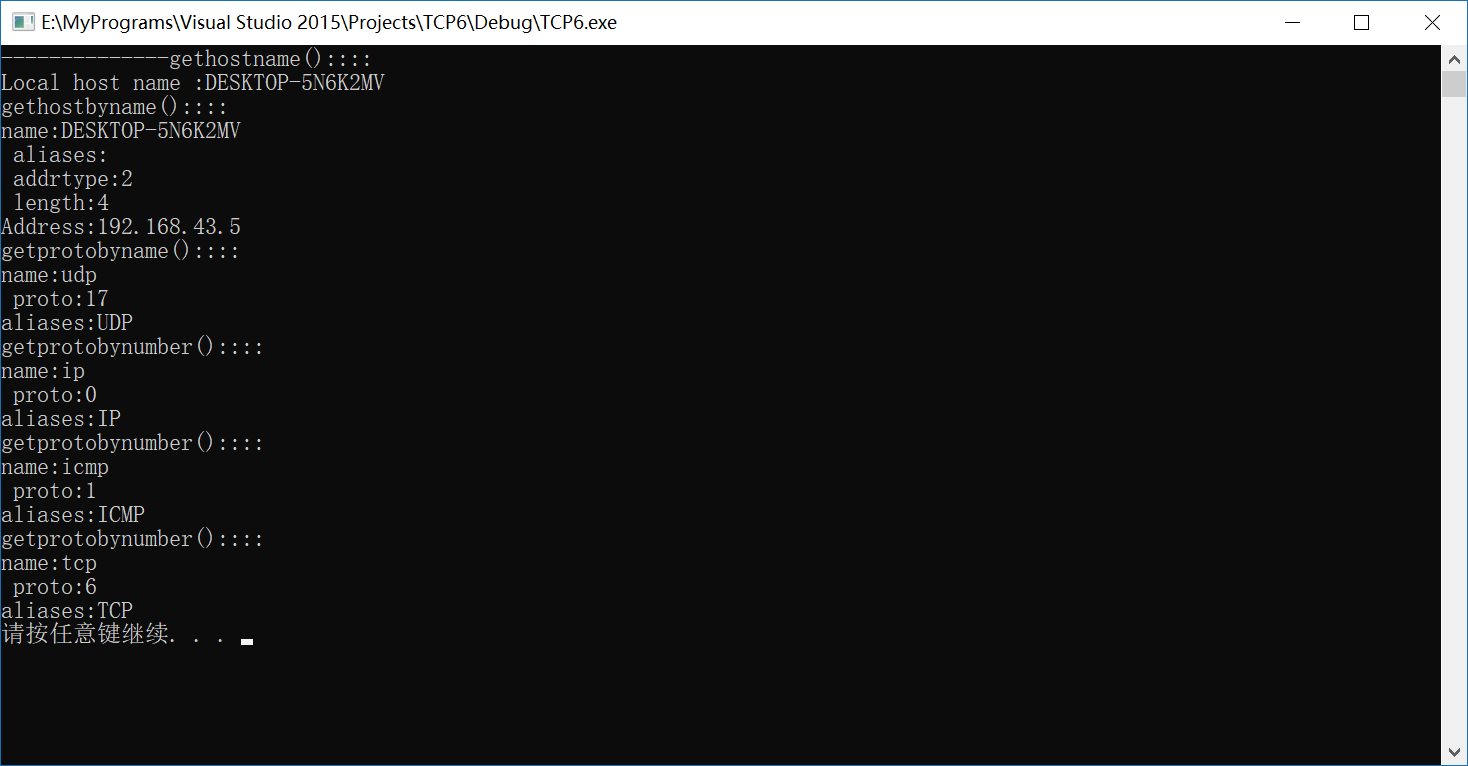
\includegraphics [width=1\textwidth]{figure//result.png}
	\caption{本地回环服务器端测试结果}\label{result}
\end{figure}

\end{spacing}
\section{问题及心得}
	\begin{itemize}
		\item 问题:经过前几次实验的积累,本次实验非常顺利,源代码编译运行一次通过,没有遇到阻碍实验进行的问题。
		\item 心得:\begin{enumerate}
			\item 实践是检验真理的唯一标准;
			\item 实验是巩固知识的最快捷径;
			\item 掌握了使用C++获取网络信息的方法;
			\item 对网络编程的理解更加深入;
			\item 精进了代码水平。
		\end{enumerate}
	\end{itemize}
\end{document}